% !Mode:: "TeX:UTF-8"
% %%%%%%%%%%%%%%%%%%%%%%%%%%%%%%%%%%%%%%%%%%%%%%%%%%%%%%%%%%%%%%%%%%%%%%%%%%%%
%% 宁波大学本科生毕业论文 LaTex 模板 V1.3, 2025/04/28
%% 作者: 宁波大学机械学院,周吕文, zhoulvwen@nbu.edu.cn
%% 
%% 关注微信 #公众号:数学模型,对话框内回复“宁大模板”下载最新版本
%%
% %%%%%%%%%%%%%%%%%%%%%%%%%%%%%%%%%%%%%%%%%%%%%%%%%%%%%%%%%%%%%%%%%%%%%%%%%%%%
%% 编译命令:xelatex -> bibtex -> xelatex -> xelatex
%%
%% 本模版将论文的各部分切割成多个 .tex 文件放在 content 文件
%% 夹中,并用 \input 命令载入到主文档 main.tex 中。
%% 
%% 论文中所用到的图片都放在 figures 文件夹中
%% 
%% 附录中所用到的代码都放在 codes 文件夹中
%%
%% 参考文献按格式整理在 refs.bib 文本文件中
%%
%% 以下宏包已加载:geometry, graphicx, fancyhdr, setspace, fontspec, xeCJK, 
%%                tikz, mfirstuc, longtable, caption, subcaption, multirow, 
%%                threeparttable,booktabs, footnotebackref, natbib, listings,
%%                amsmath, amsfonts, amssymb, bm
% %%%%%%%%%%%%%%%%%%%%%%%%%%%%%%%%%%%%%%%%%%%%%%%%%%%%%%%%%%%%%%%%%%%%%%%%%%%%

% 某些学院章标题为"第一章"这种形式,请使用 ZhChapter 选项,否则可去掉
\documentclass[ZhChapter]{NBUThesis}
\title{宁波大学本科生毕业论文 \LaTeX{} 模板}
\etitle{Undergraduate Thesis \LaTeX{} Template for Ningbo University}
\author{大模头}
\supervisor{周吕文}
\college{机械工程与力学学院}
\major{工程力学}
\class{工程力学 213 班}
\studentID{20250601}
\date{2025 年 6 月 1 日}

\begin{document}

\maketitle        % 生成封面
\commitment       % 生成承诺页
\tableofcontents  % 生成目录页

% 导入中英文摘要
 % !Mode:: "TeX:UTF-8"
\begin{abstract}
\LaTeX{}通过使用预设的模板,可以编译成格式统一的PDF文档。目前,国内多数出版社和高校仍然使用Word进行文档编辑。尽管Word功能强大且灵活,但对于新手来说,在处理格式固定的学术论文时,排版、编号、引用文献等看似简单的任务却常常带来许多困难和麻烦。特别是在需要对整篇文章进行修改时,要想达到\LaTeX{}的效率,Word用户需要具备较高的技术水平。

\begin{center}
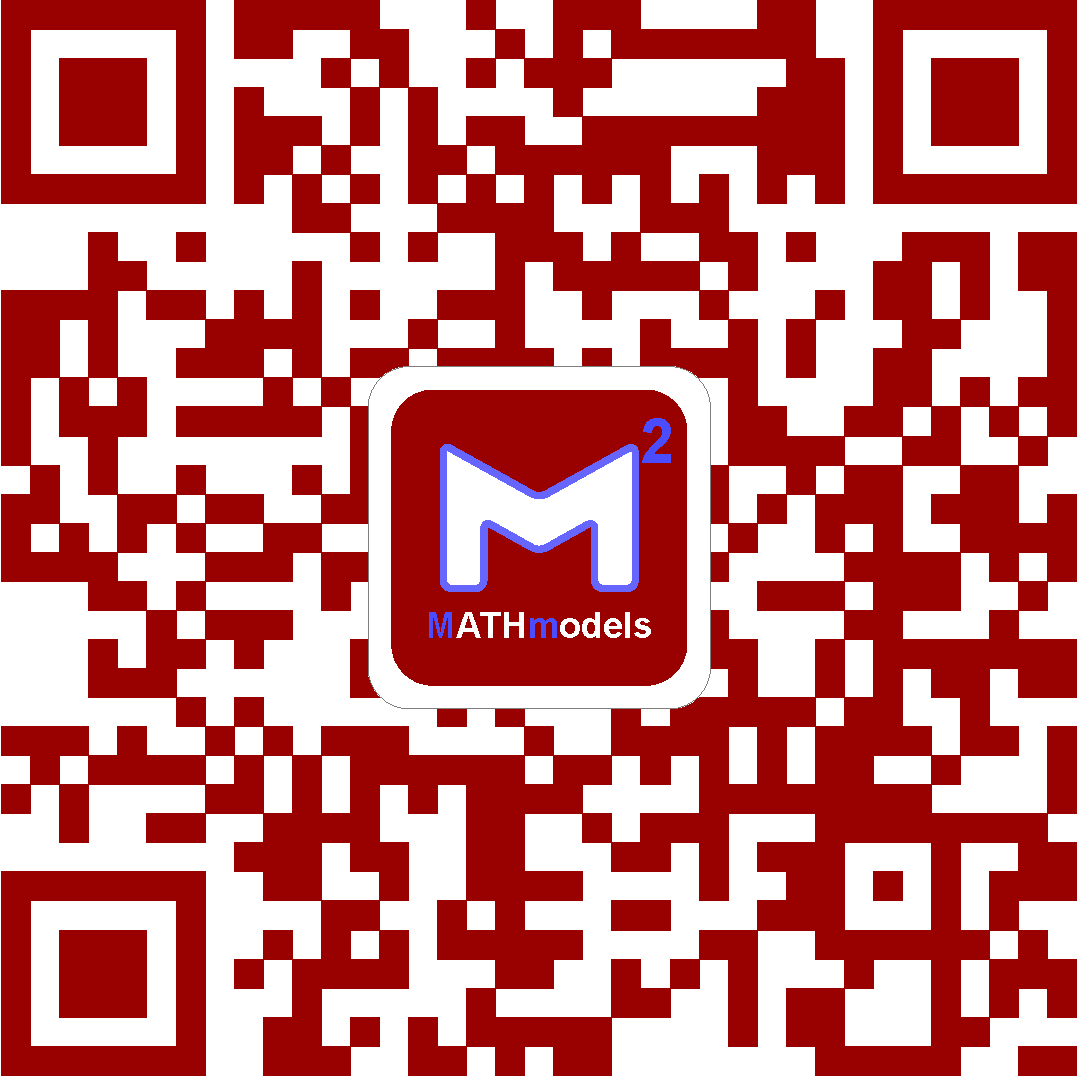
\includegraphics[width=0.3\textwidth]{mm-QR}\\

关注周老师的公众号,对话框内回复“宁大模板”下载最新模板
\end{center}

为了让研究人员能够将主要精力集中在论文写作上,许多国际期刊和高校支持使用LaTeX进行论文的撰写和提交。新手无需担心格式问题,只需使用少数标签即可生成符合要求的文档。而在需要全文格式更改时,仅需更换或修改模板文件,然后重新编译,即可获得全新的文档样式,这对于习惯使用Word的新手来说,几乎是不可思议的。

本项目旨在创建一个符合宁波大学本科生论文撰写规范的\LaTeX{}模板,以解决学位论文撰写中的格式调整问题。

\keywords{宁波大学, \LaTeX{}, 学位论文}{;}
\end{abstract}

% ----------------------------------------------------------------------------

\begin{abstractEN}
Using a pre-set \LaTeX{} template enables the compilation of PDF documents with uniform formatting. Currently, most publishers and universities in China continue to use Word for document processing. Although Word is powerful and versatile, it often presents significant challenges for beginners, especially when dealing with fixed-format academic papers. Tasks such as layout, numbering, and referencing, which seem simple, can become cumbersome. Additionally, achieving the efficiency of \LaTeX{} for comprehensive document revisions requires a high level of Word proficiency.

To allow researchers to concentrate primarily on writing, many international journals and universities support drafting and submitting papers in \LaTeX{}. Beginners do not need to be concerned about formatting details; using just a few symbolic tags can meet the required document standards. Moreover, when changes to the entire document format are needed, simply altering or updating the template file and recompiling can produce a new style of document—an incredibly advantageous process compared to using Word.

This project aims to develop a \LaTeX{} template that adheres to the writing standards for undergraduate students at Ningbo University, thereby addressing the challenges associated with formatting adjustments during thesis writing.
    
\keywords{Ningbo University, \LaTeX{}, Template}{;}
\end{abstractEN}






\mainmatter       % 正文开始

% 正文章节
% !Mode:: "TeX:UTF-8"

%为了便于查找和修改,还可以拆分文件为子章节,并通过input导入。

\chapter{模板结构}

模板文件的结构,如下表所示:
\begin{table}[ht]\centering
\begin{tabular}{r|l|l}
\hline
\multicolumn{2}{l|}{main.tex }       & 主文档,在其中填写正文  \\ \hline
content 文件夹 & abstract.tex         & 中/英文摘要、关键词     \\ \cline{2-3} \hline
content 文件夹 & content.tex          & 正文                     \\ \hline
content 文件夹 & acknowledgements.tex & 致谢                     \\ \hline
content 文件夹 & appendix.tex         & 附录                     \\ \hline
\multicolumn{2}{l|}{figures 文件夹}   & 存放图片文件            \\ \hline
\multicolumn{2}{l|}{codes 文件夹}     & 存放代码                \\ \hline
\multicolumn{2}{l|}{NBUThesis.cls}   & 定义文档格式             \\ \hline
\multicolumn{2}{l|}{refs.bib}        & 参考文献存放             \\ \hline
\multicolumn{2}{l|}{nbuthesis.bst}   & 参考文献格式             \\ \hline
\end{tabular}
\end{table}

无需也不要改变、移动上述文档的位置。

\section{使用步骤}

\begin{enumerate}
\item 进入 content 文件夹, 打开 abstract.tex 并分别填写中、英文摘要、关键词;打开 acknowledgements.tex 填写致谢;打开 content.tex 填写正文部分;打开 appendix.tex 填写附录内容。

\item 将图片放入 figures 文件夹,支持 PDF、JPG、PNG 等格式的图片,最好是 PDF 格式的矢量图。

\item 将参考文献信息录入 refs.bib,并在正文中正确引用。

\item 使用 XeLaTeX 编译。具体见 \ref{sec-compile} 节。
\end{enumerate}

\section{编译方法} \label{sec-compile}

按照 xelatex $\rightarrow$ bibtex $\rightarrow$ xelatex ($\times 2$) 的顺序编译,直接生成~pdf 文件。

% %%%%%%%%%%%%%%%%%%%%%%%%%%%%%%%%%%%%%%%%%%%%%%%%%%%%%%%%%%%%%%%%%%%%%%%%%%%%

\chapter{字体操作}
\section{字体调节}

\begin{tabular}{lllll}
\verb|\songti|    & {\songti 宋体}    &~~~&\verb|\bfseries|          & {\bfseries 粗宋体}\\
\verb|\sffamily|  & {\sffamily 黑体}  &~~~&\verb|\bfseries\sffamily| & {\bfseries\sffamily 粗黑体}\\
\verb|\ttfamily|  & {\ttfamily 楷体}  &~~~&\verb|\bfseries\kaiti|    & {\bfseries\kaiti 粗楷体}\\
%\verb|\itshape|   & {\itshape 斜宋体} &~~~&\verb|\bfseries\itshape|  & {\bfseries\itshape 粗斜宋体}\\
\end{tabular}

\section{字号调节}
%字号命令: \verb|\zihao| \index{zihao}
\begin{tabular}{ll}
\verb|\zihao{0}| &\zihao{0}  初号字 English \\
\verb|\zihao{-0}|&\zihao{-0} 小初号 English \\
\verb|\zihao{1} |&\zihao{1}  一号字 English \\
\verb|\zihao{-1}|&\zihao{-1} 小一号 English \\
\verb|\zihao{2} |&\zihao{2}  二号字 English \\
\verb|\zihao{-2}|&\zihao{-2} 小二号 English \\
\verb|\zihao{3} |&\zihao{3}  三号字 English \\
\verb|\zihao{-3}|&\zihao{-3} 小三号 English \\
\verb|\zihao{4} |&\zihao{4}  四号字 English \\
\verb|\zihao{-4}|&\zihao{-4} 小四号 English \\
\verb|\zihao{5} |&\zihao{5}  五号字 English \\
\verb|\zihao{-5}|&\zihao{-5} 小五号 English \\
\verb|\zihao{6} |&\zihao{6}  六号字 English \\
\verb|\zihao{-6}|&\zihao{-6} 小六号 English \\
\verb|\zihao{7} |&\zihao{7}  七号字 English \\
\verb|\zihao{8} |&\zihao{8}  八号字 English \\
\end{tabular}

% %%%%%%%%%%%%%%%%%%%%%%%%%%%%%%%%%%%%%%%%%%%%%%%%%%%%%%%%%%%%%%%%%%%%%%%%%%%%

\chapter{列表环境}

圆点编号
\begin{itemize}
 \item XXXXXXXXXX
 \item XXXXXXXXXX
 \item XXXXXXXXXX
\end{itemize}

数字编号
\begin{enumerate}
 \item XXXXXXXXXX
 \item XXXXXXXXXX
 \item XXXXXXXXXX
\end{enumerate}

罗马编号
\begin{enumerate}[label=(\roman*)]
 \item XXXXXXXXXX
 \item XXXXXXXXXX
 \item XXXXXXXXXX
\end{enumerate}

括号编号
\begin{enumerate}[label=(\arabic*)]
 \item XXXXXXXXXX
 \item XXXXXXXXXX
 \item XXXXXXXXXX
\end{enumerate}

半括号编号
\begin{enumerate}[label=\arabic*)]
 \item XXXXXXXXXX
 \item XXXXXXXXXX
 \item XXXXXXXXXX
\end{enumerate}

小字母编号
\begin{enumerate}[label=\alph*)]
 \item XXXXXXXXXX
 \item XXXXXXXXXX
 \item XXXXXXXXXX
\end{enumerate}

% %%%%%%%%%%%%%%%%%%%%%%%%%%%%%%%%%%%%%%%%%%%%%%%%%%%%%%%%%%%%%%%%%%%%%%%%%%%%

\chapter{公式环境}

\section{行内公式}
写在文字行中的公式称为“行内公式”,例如 $ \theta $ 是角度。行内公式使用 \verb|$  $| 包裹。

\section{行间公式}
单独成行的公式称为“行间公式”,行间公式不需要编号的可以使用 \verb|\[  \]| 包裹,例如
\[
E=mc^2
\]
其中 $E$ 是能量,$m$ 是质量,$c$ 是光速。如果希望公式带编号,并且在后文中引用可以参考下面的写法:
\begin{equation}\label{eq:energy}
E=mc^2
\end{equation}
\verb|\label{eq:energy}| 是一个标签,供交叉引用使用的。例如引用上式 \verb|\ref{eq:energy}| 的实际效果是 \ref{eq:energy}。

\section{其它公式}
多行公式有时候希望能够在特定的位置对齐,以下是其中一种处理方法。
\begin{align}
P & = UI \\
& = I^2R
\end{align}
\verb|&| 是对齐的位置, \verb|&| 可以有多个,但是每行的个数要相同。

矩阵的输入也不难。
\[
\mathbf{X} = \left(
    \begin{array}{cccc}
    x_{11} & x_{12} & \ldots & x_{1n}\\
    x_{21} & x_{22} & \ldots & x_{2n}\\
    \vdots & \vdots & \ddots & \vdots\\
    x_{n1} & x_{n2} & \ldots & x_{nn}\\
    \end{array} \right)
\]

分段函数这些可以用 \verb|case| 环境,但是它要放在数学环境里面。
\[
f(x) =
    \begin{cases}
        0 &  x \text{为无理数} ,\\
        1 &  x \text{为有理数} .
    \end{cases}
\]
在数学环境里面,字体用的是数学字体,一般与正文字体不同。假如要公式里面有个别文字,则需要把这部分放在 \verb|text| 环境里面,即 \verb|\text{文本环境}| 。

公式中个别需要加粗的字母可以用 \verb|$\bm{math symbol}$| 。如 $ \alpha a\bm{\alpha a} $ 。

以上仅简单介绍了基础的使用,对于更复杂的需求,可以阅读相关的宏包手册,如 \href{http://texdoc.net/texmf-dist/doc/latex/amsmath/amsldoc.pdf}{amsmath}。

希腊字母这些如果不熟悉,可以去查找符号文件 \href{http://mirrors.ctan.org/info/symbols/comprehensive/symbols-a4.pdf}{symbols-a4.pdf} ,也可以去 \href{http://detexify.kirelabs.org/classify.html}{detexify} 网站手写识别。另外还有数学公式识别软件 \href{https://mathpix.com/}{mathpix} 。

% %%%%%%%%%%%%%%%%%%%%%%%%%%%%%%%%%%%%%%%%%%%%%%%%%%%%%%%%%%%%%%%%%%%%%%%%%%%%

\chapter{图表环境}

\section{图环境}
图片可以分为矢量图与位图。位图推荐使用 \verb|jpg,png| 这两种格式,避免使用 \verb|bmp| 这类图片,容易出现图片插入失败这样情况的发生。矢量图一般有 \verb|pdf,eps| ,推荐使用 \verb|pdf|  格式的图片,尽量不要使用 \verb|eps| 图片,理由相同。

下面是一个插图的示例代码。
\begin{figure}[!htb]
  \centering
  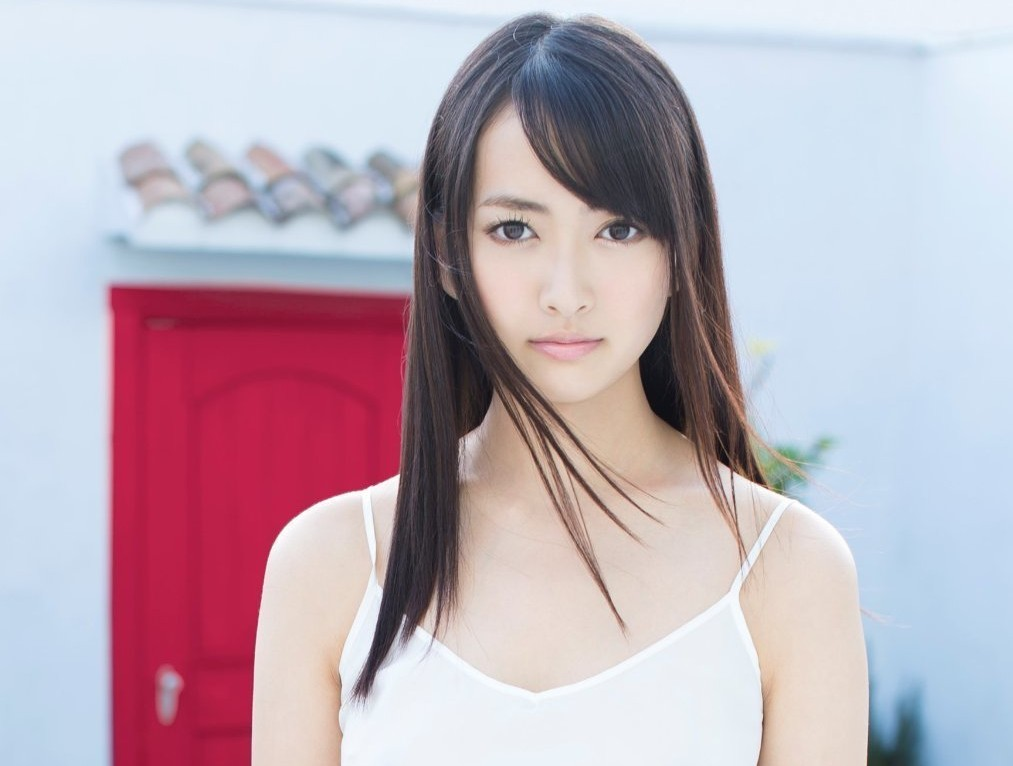
\includegraphics[width=0.4\textwidth]{Risa.jpg}
  \caption{一个纯洁漂亮的女孩子}
  \label{fig:Risa}
\end{figure}
注意 \verb|figure| 环境是一个浮动体环境,图片的最终位置可能会跑动。\verb|[!h]| 中的 \verb|h| 是 here 的意思, \verb|!| 表示忽略一些浮动体的严格规则。另外里面还可以加上 \verb|btp| 选项,它们分别是 bottom, top, page 的意思。只要这几个参数在花括号里面,作用是不分先后顺序的。page 在这里表示浮动页。\verb|width=0.6\textwidth| 表示设计图片的宽度为文本的 0.6 倍。\verb|\label{fig:Risa}| 是一个标签,供交叉引用使用的。例如引用图片 \verb|\ref{fig:Risa}| 的实际效果是 \ref{fig:Risa}。图片是自动编号的,比起手动编号,它更加高效。\verb|label| 要确保唯一,命名方式推荐用图片的命名方式。

图片并排的需求解决方式多种多样,下面用 \verb|minipage| 环境来展示一个简单的例子。注意,以下例子用到了 \verb|subcaption| 命令,需要加载 subcaption 宏包。
\begin{figure}[!htb]
    \centering
    \begin{minipage}[c]{0.32\textwidth}
        \centering
        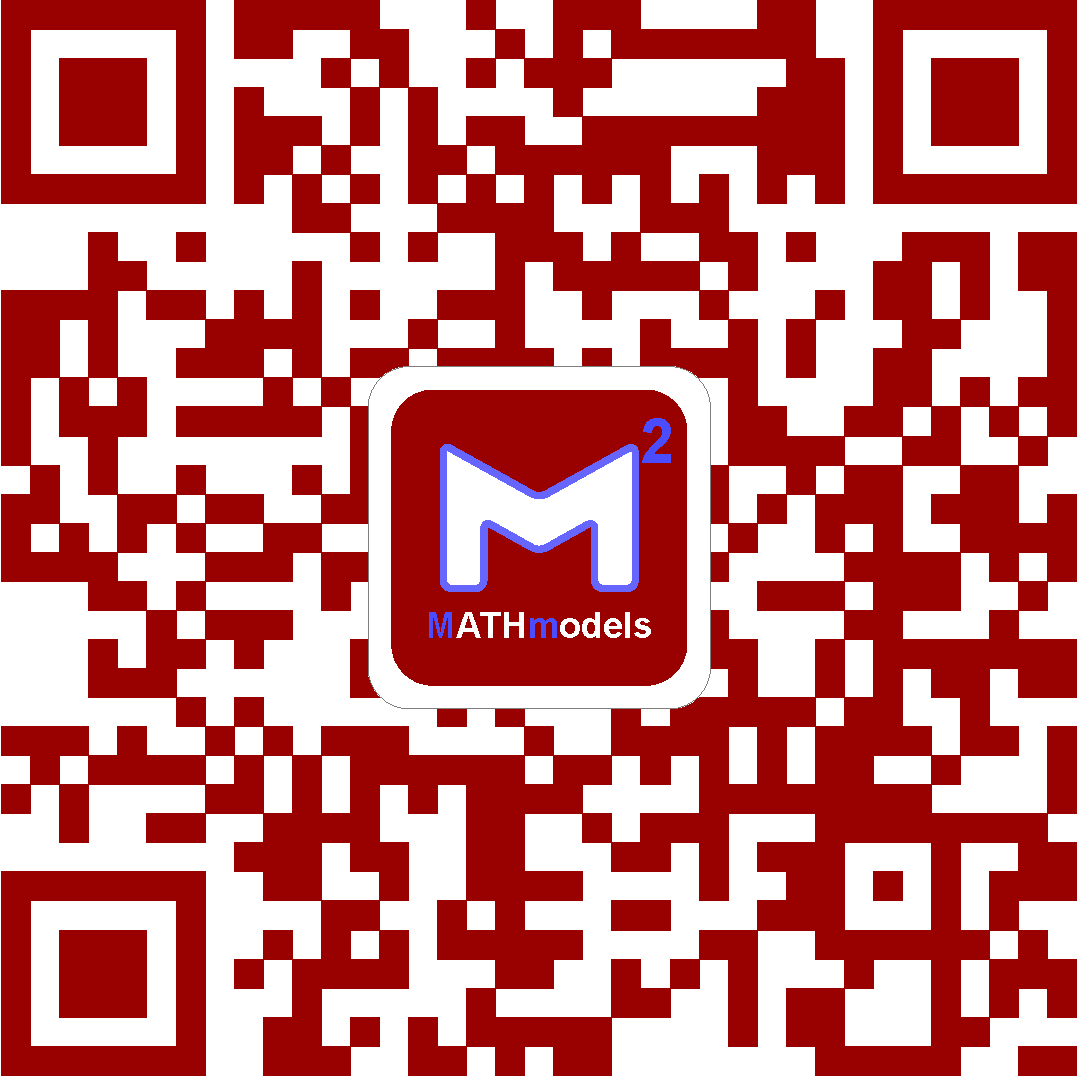
\includegraphics[width=0.7\textwidth]{mm-QR.pdf}
        \subcaption{数学模型微信公众号}
        \label{fig:QR-mm}
    \end{minipage}
    \begin{minipage}[c]{0.32\textwidth}
        \centering
        
\includegraphics[width=0.7\textwidth]{hi-QR.pdf}
        \subcaption{HiMCM 微信公众号}
        \label{fig:QR-hi}
    \end{minipage}
    \begin{minipage}[c]{0.32\textwidth}
        \centering
        
\includegraphics[width=0.7\textwidth]{km-QR.pdf}
        \subcaption{大模头微信号}
        \label{fig:QR-km}
    \end{minipage}
    \caption{周老师(本模板作者)的公众号。关注“数学模型”,对话框内回复“宁大模板”下载最新版}
    \label{fig:QR}
\end{figure}
这相当于整体是一张大图片,大图片引用是 \ref{fig:QR},子图引用别分是 \ref{fig:QR-mm}、\ref{fig:QR-hi}、\ref{fig:QR-km}。当然,你也可以将两个独立的图片并排,并分别编号,具体如图 \ref{fig:problem} 和 \ref{fig:map},这两张图来源于周老师的公众号文章:\href{https://mp.weixin.qq.com/s/uI-NiR-1rdzeKxjOOUzqlw}{被“天屎”击中的概率有多大?}\cite{nbubirds}。

\begin{figure}[!htb]
    \centering
    \begin{minipage}[c]{0.45\textwidth}
        \centering
        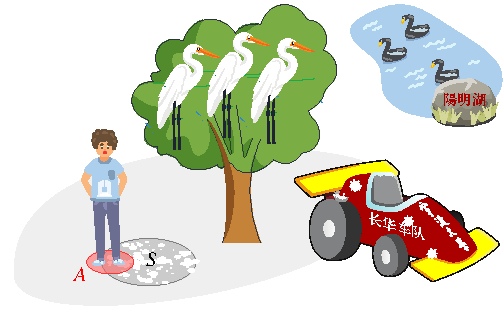
\includegraphics[width=\textwidth]{problem.pdf}
        \caption{鸟屎区域和人在地面投影区域的定义}\label{fig:problem}
    \end{minipage}
    \begin{minipage}[c]{0.075\textwidth}
         ~% 两图之间空点距离
    \end{minipage}
    \begin{minipage}[c]{0.45\textwidth}
        \centering
        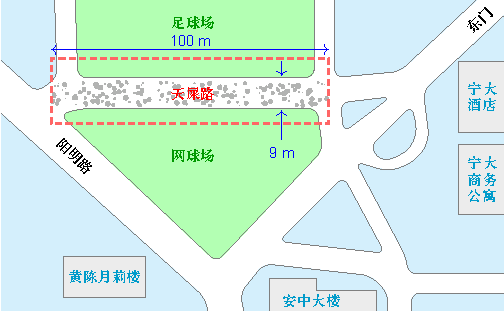
\includegraphics[width=\textwidth]{map.pdf}
        \caption{宁波大学其中一条天屎路示意图}
        \label{fig:map}
    \end{minipage}
\end{figure}


\section{表环境}
表格应具有三线表格式,因此常用 booktabs宏包,其标准格式如 \ref{tab:mytab} 所示。
\begin{table}[!htbp]
    \caption{标准三线表格}\label{tab:mytab} \centering
    \begin{tabular}{ccccc}
        \toprule[1.5pt]
        $D$(in) & $P_u$(lbs) & $u_u$(in) & $\beta$ & $G_f$(psi.in)\\
        \midrule[1pt]
        5 & 269.8 & 0.000674 & 1.79 & 0.04089\\
        10 & 421.0 & 0.001035 & 3.59 & 0.04089\\
        20 & 640.2 & 0.001565 & 7.18 & 0.04089\\
        \bottomrule[1.5pt]
    \end{tabular}
\end{table}

table 环境是一个将表格嵌入文本的浮动环境。tabular 环境的必选参数由每列对应一个格式字符所组成:\verb|c| 表示居中,\verb|l| 表示左对齐,\verb|r| 表示右对齐,其总个数应与表的列数相同。此外,\verb|@{文本}| 可以出现在任意两个上述的列格式之间,其中的文本将被插入每一行的同一位置。表格的各行以 \verb|\\| 分隔,同一行的各列则以\&分隔。 \verb|\toprule| 、\verb|\midrule| 和 \verb|\bottomrule| 三个命令是由booktabs宏包提供的,其中 \verb|\toprule| 和 \verb|\bottomrule| 分别用来绘制表格的第一条(表格最顶部)和第三条(表格最底部)水平线,\verb|\midrule| 用来绘制第二条(表头之下)水平线,且第一条和第三条水平线的线宽为 1.5pt,第二条水平线的线宽为 1pt 。引用方法与图片的相同。非三线表参考表 \ref{tab:Table-example}。
\begin{table}[!htb]
\centering
\caption{Table example}\label{tab:Table-example}
\begin{tabular}{|c|c|c|c|c|}
\hline 
 & AAAAAA & BBBBBB & CCCCCC & DDDDDD\tabularnewline
\hline 
XXX & 1 & 2 & 3 & 4\tabularnewline
\hline 
YYY & 5 & 6 & 7 & 8\tabularnewline
\hline 
\end{tabular}
\end{table}

% %%%%%%%%%%%%%%%%%%%%%%%%%%%%%%%%%%%%%%%%%%%%%%%%%%%%%%%%%%%%%%%%%%%%%%%%%%%%


\chapter{参考文献与脚注}

\section{参考文献与引用}

参考文献对于一篇正式的论文来说是必不可少的,在建模中重要的参考文献当然应该列出。\LaTeX{}在这方面的功能也是十分强大的,下面进介绍一个比较简单的参考文献制作方法。有兴趣的可以学习 \verb|bibtex| 或 \verb|biblatex| 的使用。

这是一个简单的引用 \cite{zhangkun1994,zhukezhen1973},用 \verb|\cite{bibkey}| 来完成。如果不想上标,可用 \verb|\Cite{bibkey}| 实现(注意,"C"是大写),例如\Cite{scitor2000project}。


\section{脚注}

利用 \verb|\footnote{具体内容}| 可以生成脚注\footnote{脚注可以补充说明一些东西}。


% 参考文献
\addcontentsline{toc}{chapter}{参考文献}
\bibliographystyle{nbuthesis}
\bibliography{refs} 

% 致谢
 % !Mode:: "TeX:UTF-8"
\begin{acknowledgements}

首先,我要感谢周吕文老师。他的这份\LaTeX{}模板对我写毕业论文帮助很大。周老师长相帅气、为人和善,多才多艺。周老师不仅精通 Python,JavaScrpt,HTML,VB,C++ 等多种语言,还熟悉 Ubuntu、Fedora、CentOS、openSUSE、MacOS、Windows 等多种操作系统。此外,周老师还对搬砖、砌墙、刮大白、修理抽油烟机、通下水做防水、拔牙、割包皮、丰胸、算命、按摸、摄影、卫星轨道修正、火星探测器维修、太阳黑子观测、考古发掘、石油勘探、视频剪辑、配音、考研辅导、滴滴快车、送美团外卖、代写小学生作业、代开家长会、解偏微分方程、婚礼司仪、产后护理、心理咨询、殡葬服务、代练游戏账号、自媒体运营、民事诉讼、离婚调查、企业财务、讨债等领域也有广泛涉猎。

其次,我要感谢我的导师。他放下神圣的师道尊严,以朋友的身份告诉我怎样完成这篇论文。他告诉我如何搜集资料;他告诉我如何快捷地找到相关论文;他告诉我哪个学校的网站有本专业的硕士、博士论文;他指导我如何利用手头上的论文取舍嫁接整合。本论文的完成,离不开他的悉心指导和孜孜不倦地教诲。

最后,我要感谢我的女朋友,在我 22 年的生命中始终没有出现过,让我得以专心于学术,顺利完成本科论文。
\end{acknowledgements}


% 附录
\appendix
 % !Mode:: "TeX:UTF-8"
\chapter{补充内容}
\section{程序}\label{sec:cod}

\lstinputlisting[language=matlab,caption={一段 MATLAB 程序},label=cod:example]{codes/example.m}
\lstinputlisting[language=C++,caption={一段 C++ 程序},label=cod:hellow]{codes/example.cpp}
\lstinputlisting[language=python, caption={一段 python 程序},label=cod:fre]{codes/example.py}

\section{长表格}
\begin{longtable}{c|c|c}
\caption{数据长表格}\\
\hline 
AAAAAAAAAAAAAAAAA & BBBBBBBBBBBBBBBBB & CCCCCCCCCCCCCCCCC\\
\endfirsthead
\hline 
AAAAAAAAAAAAAAAAA & BBBBBBBBBBBBBBBBB & CCCCCCCCCCCCCCCCC\\
\hline 
\endhead
\hline 
 1 &  & \\
 2 &  & \\
 3 &  & \\
 4 &  & \\
 5 &  & \\      \hline 
 6 &  & \\
 7 &  & \\
 8 &  & \\
 9 &  & \\
10 &  & \\     \hline 
11 &  & \\
12 &  & \\
13 &  & \\
14 &  & \\
15 &  & \\     \hline 
16 &  & \\
17 &  & \\
18 &  & \\
19 &  & \\
20 &  & \\
\hline 
\end{longtable}

\end{document}
